\documentclass[11pt,a4paper]{article}
\newcommand{\intestazione}{Trimero ad anello --- 7. La dinamica sotto rumore}
% =====================================================================
%  Preambolo comune ai documenti sul dimero (serie "che cosa abbiamo fatto")
%  Incluso con % =====================================================================
%  Preambolo comune ai documenti sul dimero (serie "che cosa abbiamo fatto")
%  Incluso con % =====================================================================
%  Preambolo comune ai documenti sul dimero (serie "che cosa abbiamo fatto")
%  Incluso con \input{preambolo_dimero} subito dopo \documentclass.
% =====================================================================
\usepackage[T1]{fontenc}
\usepackage[utf8]{inputenc}
\usepackage[main=italian,provide=*]{babel}
\usepackage{amsmath,amssymb,mathtools}
\usepackage{graphicx}
\usepackage{booktabs}
\usepackage{colortbl}
\usepackage{xcolor}
\usepackage{geometry}
\usepackage{placeins}
\usepackage{caption}
\usepackage{enumitem}
\usepackage{fancyhdr}
\usepackage{needspace}
\usepackage{tikz}
\usetikzlibrary{arrows.meta,positioning,shapes.geometric,calc,fit,backgrounds}
\usepackage{hyperref}
\hypersetup{colorlinks=true,linkcolor=blu,citecolor=blu,urlcolor=blu}

\geometry{margin=2.5cm}

% --- colori coerenti con quelli delle figure (palette Okabe-Ito)
\definecolor{blu}{HTML}{0072B2}
\definecolor{arancio}{HTML}{E69F00}
\definecolor{verdes}{HTML}{009E73}
\definecolor{rossos}{HTML}{D55E00}
\definecolor{violas}{HTML}{CC79A7}
\definecolor{grigetto}{HTML}{E8E8E8}

\captionsetup{font=small,labelfont=bf,width=0.92\textwidth}

\pagestyle{fancy}
\fancyhf{}
\fancyhead[L]{\small\itshape\intestazione}
\fancyhead[R]{\small\thepage}
\renewcommand{\headrulewidth}{0.3pt}

% --- notazione
\newcommand{\ket}[1]{\lvert #1\rangle}
\newcommand{\bra}[1]{\langle #1 \rvert}
\newcommand{\media}[1]{\langle #1 \rangle}
\newcommand{\vs}[1]{\mathbf{s}_{#1}}

% --- riquadro "in una riga": il messaggio da portare a casa
\newcommand{\messaggio}[1]{%
  \begin{center}
  \begin{minipage}{0.93\textwidth}
  \setlength{\fboxsep}{9pt}%
  \colorbox{grigetto}{\begin{minipage}{\dimexpr\textwidth-2\fboxsep}
  \small\textbf{In una riga.}\enspace #1
  \end{minipage}}
  \end{minipage}
  \end{center}
}

% --- riquadro "come lo sappiamo": la verifica numerica dietro un'affermazione
\newcommand{\verifica}[1]{%
  \begin{center}
  \begin{minipage}{0.93\textwidth}
  \small\textcolor{verdes}{\rule{2.2em}{1.1pt}}\enspace
  \textcolor{verdes}{\textbf{Come lo sappiamo.}}\enspace #1
  \end{minipage}
  \end{center}
  \medskip
}
 subito dopo \documentclass.
% =====================================================================
\usepackage[T1]{fontenc}
\usepackage[utf8]{inputenc}
\usepackage[main=italian,provide=*]{babel}
\usepackage{amsmath,amssymb,mathtools}
\usepackage{graphicx}
\usepackage{booktabs}
\usepackage{colortbl}
\usepackage{xcolor}
\usepackage{geometry}
\usepackage{placeins}
\usepackage{caption}
\usepackage{enumitem}
\usepackage{fancyhdr}
\usepackage{needspace}
\usepackage{tikz}
\usetikzlibrary{arrows.meta,positioning,shapes.geometric,calc,fit,backgrounds}
\usepackage{hyperref}
\hypersetup{colorlinks=true,linkcolor=blu,citecolor=blu,urlcolor=blu}

\geometry{margin=2.5cm}

% --- colori coerenti con quelli delle figure (palette Okabe-Ito)
\definecolor{blu}{HTML}{0072B2}
\definecolor{arancio}{HTML}{E69F00}
\definecolor{verdes}{HTML}{009E73}
\definecolor{rossos}{HTML}{D55E00}
\definecolor{violas}{HTML}{CC79A7}
\definecolor{grigetto}{HTML}{E8E8E8}

\captionsetup{font=small,labelfont=bf,width=0.92\textwidth}

\pagestyle{fancy}
\fancyhf{}
\fancyhead[L]{\small\itshape\intestazione}
\fancyhead[R]{\small\thepage}
\renewcommand{\headrulewidth}{0.3pt}

% --- notazione
\newcommand{\ket}[1]{\lvert #1\rangle}
\newcommand{\bra}[1]{\langle #1 \rvert}
\newcommand{\media}[1]{\langle #1 \rangle}
\newcommand{\vs}[1]{\mathbf{s}_{#1}}

% --- riquadro "in una riga": il messaggio da portare a casa
\newcommand{\messaggio}[1]{%
  \begin{center}
  \begin{minipage}{0.93\textwidth}
  \setlength{\fboxsep}{9pt}%
  \colorbox{grigetto}{\begin{minipage}{\dimexpr\textwidth-2\fboxsep}
  \small\textbf{In una riga.}\enspace #1
  \end{minipage}}
  \end{minipage}
  \end{center}
}

% --- riquadro "come lo sappiamo": la verifica numerica dietro un'affermazione
\newcommand{\verifica}[1]{%
  \begin{center}
  \begin{minipage}{0.93\textwidth}
  \small\textcolor{verdes}{\rule{2.2em}{1.1pt}}\enspace
  \textcolor{verdes}{\textbf{Come lo sappiamo.}}\enspace #1
  \end{minipage}
  \end{center}
  \medskip
}
 subito dopo \documentclass.
% =====================================================================
\usepackage[T1]{fontenc}
\usepackage[utf8]{inputenc}
\usepackage[main=italian,provide=*]{babel}
\usepackage{amsmath,amssymb,mathtools}
\usepackage{graphicx}
\usepackage{booktabs}
\usepackage{colortbl}
\usepackage{xcolor}
\usepackage{geometry}
\usepackage{placeins}
\usepackage{caption}
\usepackage{enumitem}
\usepackage{fancyhdr}
\usepackage{needspace}
\usepackage{tikz}
\usetikzlibrary{arrows.meta,positioning,shapes.geometric,calc,fit,backgrounds}
\usepackage{hyperref}
\hypersetup{colorlinks=true,linkcolor=blu,citecolor=blu,urlcolor=blu}

\geometry{margin=2.5cm}

% --- colori coerenti con quelli delle figure (palette Okabe-Ito)
\definecolor{blu}{HTML}{0072B2}
\definecolor{arancio}{HTML}{E69F00}
\definecolor{verdes}{HTML}{009E73}
\definecolor{rossos}{HTML}{D55E00}
\definecolor{violas}{HTML}{CC79A7}
\definecolor{grigetto}{HTML}{E8E8E8}

\captionsetup{font=small,labelfont=bf,width=0.92\textwidth}

\pagestyle{fancy}
\fancyhf{}
\fancyhead[L]{\small\itshape\intestazione}
\fancyhead[R]{\small\thepage}
\renewcommand{\headrulewidth}{0.3pt}

% --- notazione
\newcommand{\ket}[1]{\lvert #1\rangle}
\newcommand{\bra}[1]{\langle #1 \rvert}
\newcommand{\media}[1]{\langle #1 \rangle}
\newcommand{\vs}[1]{\mathbf{s}_{#1}}

% --- riquadro "in una riga": il messaggio da portare a casa
\newcommand{\messaggio}[1]{%
  \begin{center}
  \begin{minipage}{0.93\textwidth}
  \setlength{\fboxsep}{9pt}%
  \colorbox{grigetto}{\begin{minipage}{\dimexpr\textwidth-2\fboxsep}
  \small\textbf{In una riga.}\enspace #1
  \end{minipage}}
  \end{minipage}
  \end{center}
}

% --- riquadro "come lo sappiamo": la verifica numerica dietro un'affermazione
\newcommand{\verifica}[1]{%
  \begin{center}
  \begin{minipage}{0.93\textwidth}
  \small\textcolor{verdes}{\rule{2.2em}{1.1pt}}\enspace
  \textcolor{verdes}{\textbf{Come lo sappiamo.}}\enspace #1
  \end{minipage}
  \end{center}
  \medskip
}


\title{\bfseries Più passi non è sempre meglio\\[2pt]
\large Documento 7 --- il compromesso Trotter/rumore, due scenari}
\author{Samuele Schiavi \\ \small Tesi triennale in Fisica, Università di Parma
--- Relatore: Prof.\ Alessandro Chiesa}
\date{}

\begin{document}
\maketitle
\thispagestyle{fancy}

\section{Il compromesso che il sistema chiuso non poteva mostrare}

Nella Parte 1 (Documento 3), l'errore di Trotter scende monotonamente con
$N$: più passi, meglio è, unico costo la profondità del circuito. Sotto
rumore questo non è più vero --- ogni passo aggiunge $15$ CNOT rumorosi
(Documento 3, costo dopo compilazione ottimizzata). Esiste un $N^*$ che
massimizza la fedeltà rumorosa, né il più piccolo né il più grande.

\section{Due scenari, non uno}

A differenza del dimero (un solo punto di lavoro per i cinque stadi
principali della Parte 2 --- un secondo punto compare solo nel Documento
10, per verificare la generalità dell'estensione noise-aware), qui
si trattano \textbf{entrambi} gli scenari già distinti nella Parte 1:

\begin{itemize}[leftmargin=1.8em,itemsep=3pt]
\item \textbf{Scenario A} ($b/J=2.4$, $D/J=0.15$): preparazione VQE
($W$-2q.6, Scenario A della Parte 1), poi $N$ passi di Trotter.
\item \textbf{Scenario B} ($R_0$: $b/J=0.05$, $D/J=1.93$): nessuna
preparazione, si parte da $\ket{000}$ --- lo stesso schema della
dimostrazione Trotter di Parte 1.
\end{itemize}

\paragraph{Perché tenere entrambi: non è ridondanza, isolano due cose
diverse.} A Scenario A, lo stato che entra nel circuito di Trotter è
l'uscita della preparazione VQE rumorosa (Documento 6, $\mathcal
F\approx0.970$) --- quindi la curva $F(N)$ lì riflette \emph{due} sorgenti
di errore sovrapposte e non separabili guardando solo quella curva:
l'imperfezione della preparazione, e l'errore di Trotter più rumore di
gate sul circuito che segue. A $R_0$, si parte da $\ket{000}$ --- zero
gate di preparazione, zero rumore di preparazione. La curva $F(N)$ a
$R_0$ mostra quindi \emph{solo} l'effetto di Trotter più rumore di gate,
isolato dalla domanda ``quanto ha già perso la preparazione''. È l'unico
punto, in tutta questa Parte 2, dove quell'isolamento è possibile ---
in ogni altro documento (6, 8, 9, 10, 11) la preparazione VQE è sempre
presente, e i due effetti restano mescolati. Il confronto fra le due
curve della Fig.~\ref{fig:FvsN} non è quindi solo ``due esempi diversi
dello stesso fenomeno'': è l'unico modo, in questa serie, di vedere cosa
farebbe il solo Trotter rumoroso senza il contributo della preparazione.

\begin{figure}[htbp]
\centering
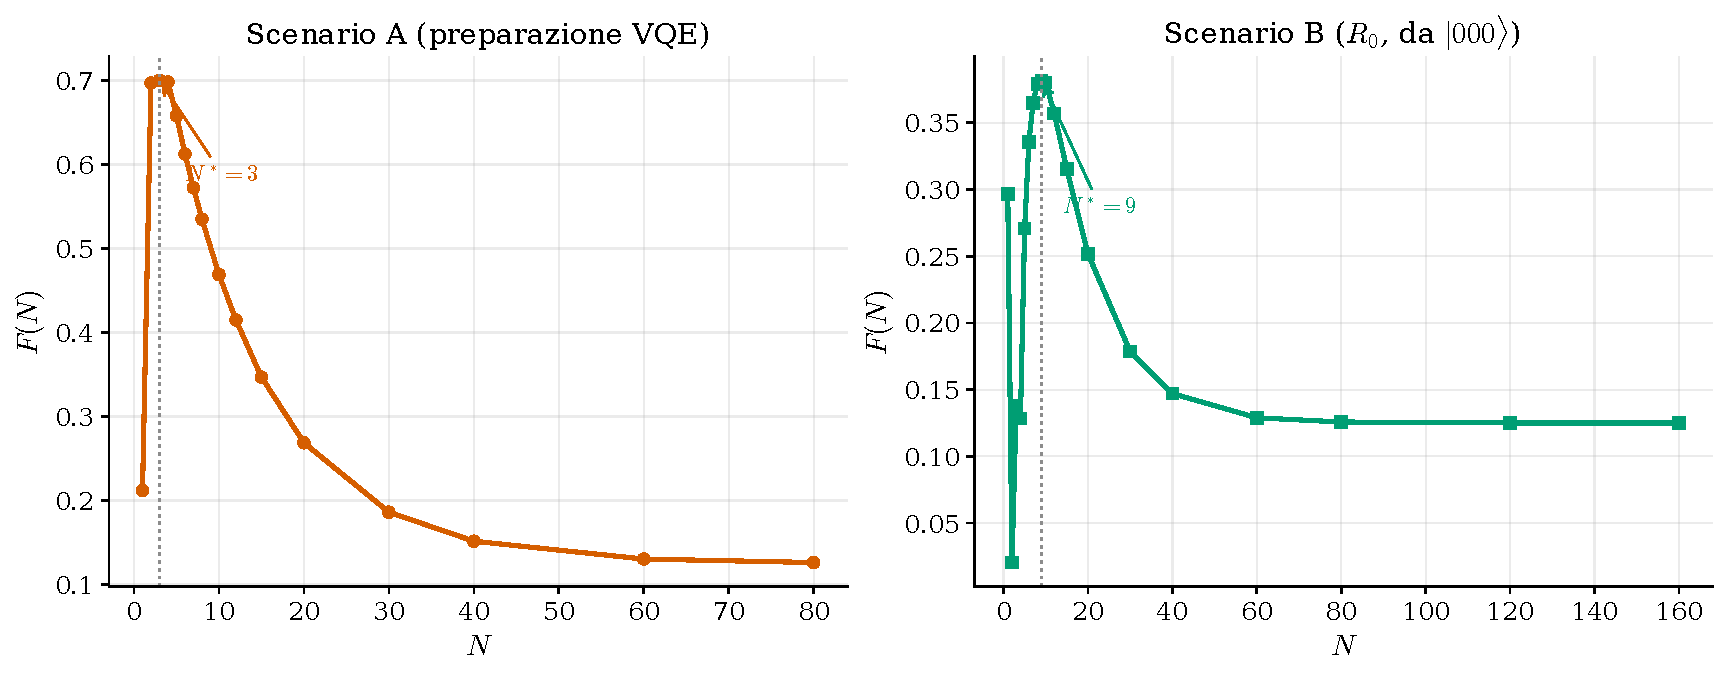
\includegraphics[width=\textwidth]{figure/fig_passo3_F_vs_N_anello}
\caption{Fedeltà rumorosa $F(N)$ rispetto allo stato bersaglio fisico, i
due scenari a confronto. \textbf{Sinistra}: Scenario A, $N^*=3$.
\textbf{Destra}: Scenario B, $N^*=9$ --- una curva più articolata, con un
minimo locale marcato attorno a $N=2$--$3$ prima di risalire al vero
massimo.}
\label{fig:FvsN}
\end{figure}
\FloatBarrier

\verifica{$N^*_A=3$, $F(N^*)=0.700335$; $N^*_B=9$, $F(N^*)=0.381896$.
Entrambi coincidono esattamente con i valori già stabiliti e verificati
indipendentemente in una sessione precedente di questo stesso progetto.}

\section{Una trappola già incontrata ed evitata}

Come sul dimero, transpilare l'\emph{intero} circuito (preparazione più
$N$ passi) a un livello di ottimizzazione alto collassa i passi identici
in un circuito a costo costante, cancellando silenziosamente la dipendenza
da $N$. Evitato transpilando una volta il singolo passo e ripetendo il
blocco già compilato --- qui con una complicazione in più rispetto al
dimero: anche il singolo passo, per l'anello, ha una struttura interna a
due livelli (scambio e DM, ciascuno spezzato sui tre legami, Documento 3)
che va transpilata come blocco unico, non gate per gate.

\section{Perché una griglia $N$ troppo rada è pericolosa}

Un avvertimento concreto, non teorico: la prima stima di $N^*_B$ per lo
Scenario B, con una griglia troppo grezza (che saltava $N=9$), aveva dato
$N^*_B=10$ --- un valore poi corretto quando lo scan sui parametri di
rumore (Documento 9) ha richiesto una griglia più fine. La Fig.~\ref{fig:FvsN}
usa già la griglia corretta.

\messaggio{Il minimo locale della curva B, attorno a $N=2$, è la stessa
fisica del ``minimo non perturbativo'' già visto sul dimero (Documento 7
gemello): a pochi passi, l'errore di Trotter può temporaneamente
\emph{aumentare} prima che il guadagno di accuratezza prenda il sopravvento
--- non un artefatto del rumore, una proprietà della dinamica stessa.}

\section{Cosa non entra in questa fedeltà}

Nessun readout è coinvolto in $F(N)$: è calcolata direttamente
sull'operatore densità, nessuna misura, nessuno shot. È per questo che i
numeri di questo documento sono identici, cifra per cifra, a quelli già
stabiliti prima che questa serie narrativa venisse scritta --- a differenza
dei Documenti 8--11, dove il passaggio al readout genuinamente campionato
introduce un margine di errore statistico da dichiarare esplicitamente.

\end{document}
